% !TEX root = MasterThesis.tex

\chapter{Case Study: Driver Development in Linux and Zircon}\label{ch:case-study}
Device drivers are an integral part of operating systems and require a good knownledge about the peripheral device and its controller, the hardware interface between device and computer and the target operating system from the programmer.
The fundamental operating system principles and their realization were already established in the previous chapter.
But the question of what a device driver actually is and its responsibility was not discussed so far.
Therefore, answering this questions is a valid entry point to the actual case study about the driver models in Linux and Zircon and the exemplarily device driver development.

A device driver's main purpose is providing an abstraction between user applications and peripheral devices\cite{glatz2015betriebssysteme}.
A common programmer should not have to think about the way a specific device is controlled.
Especially as even devices from the same type differ in the exact way the are managed, it would require too much knowledge in applications and make them very error-prone.
Thus, it is the task of a driver as a part of an operating system to 
\begin{itemize}
    \item define an abstraction of a device to the system,
    \item do the connection between applications and a certain peripherals, 
    \item initialize the peripheral controler and the device if it is needed,
    \item query the device state from the controller,
    \item log events,
    \item provide a consistent \ac{api} for all devices from the same type to the user,
    \item receive abstract application requests and translate them to commands which can be submitted to the device and
    \item transfer data from and to the device\cite{glatz2015betriebssysteme},~\cite{tanenbaum-modern-operating-systems}.
\end{itemize}
%
Driver development is very operating system dependent and has wide-ranging consequeces.
While the decision if drivers are located in user or kernel space goes alongside with the choice for an architecture, remain some further questions.
Some of them are about the way and point in time a driver is attached to the operating system.
For example if the driver must be known at compile time or if it is possible to attach it later, e.g.\ during runtime\cite{tanenbaum-modern-operating-systems}.
In any case, each system should provide a unified but extensible device driver interface which supports various device types, even for those that were non-existing at the time the operating system was designed\cite{glatz2015betriebssysteme}.
The design of the interface could be specific to each device typ or standardized for all drivers\cite{tanenbaum-modern-operating-systems}.
Furthermore, in almost every operating system specific driver model, it has to be ensured a driver is \textit{reentrant}, which means a running driver must be safe if it is called from several processes at the same time, and also still safe if peripheral devices become added or removed while the computer is still running\cite{tanenbaum-modern-operating-systems}.
In order to avoid re-developing or duplicating driver parts that remain the same for devices of the same type are device drivers often modelled and implemented as a hierarchical or layered model.
A possibility is to split into a logical and a physical layer.
The logical one contains driver functionality which remains consistent between same typed devices while the physical layer only takes care of device specific functionality\cite{tanenbaum-modern-operating-systems} 

% \section{Driver Models}
  
\section{Linux Driver Model}
\subsubsection*{Driver Types}
As already mentioned, drivers do most of all an abstraction of the communication with \ac{io} peripherals.
To do so, Linux provides more ways than widely known.
The first one is via \textit{direct hardware access} as \textit{user-space driver}.
As known from the previous sections are the most \ac{io} respectively driver related operations privileged.
But Linux offers a way for common user applications (userspace) to access hardware without a classical driver using this possibility.
It is, above all, used for video drivers which are incorporated into the \textit{X.Org display server}.
In order to obtain the neccessary rights are two systemcalls needed: \texttt{iopl()} to change the privileged level and \texttt{ioperm()} to set the \ac{io} port permissions.
These calls can only be done by a privileged Linux user, the \textit{root} user.
Compared to other options to access peripheral hardware, this one has the disadvantage that interrupts are to available at all and the user software may run into issues with demand paging.
So this way is maybe slower than a device driver in kernelspace, but for some tasks, like the already named \textit{X.Org server} is it more meaningful than a kernel driver\cite{lfd430},~\cite{glatz2015betriebssysteme}.

Another widely unknown and \ac{cpu} specific way to perform \ac{io} operations is using \textit{minimal operating system support} to access serial interfaces on x86-based \acp{cpu}.
In doing so, the kernel does not know anything about the exact device but about its \ac{io} interface\cite{glatz2015betriebssysteme}.
Thus, this variant is not handled further.
Instead, this work will focus on \ac{io} drivers in \textit{kernel-space}, the most common way device drivers in Linux are written.
This kind of driver is a part of the kernel's address space, running in the \ac{cpu}'s kernel mode and thus privileged.
User applications can access kernel drivers and thus the devices via common file operations like \texttt{open()}, \texttt{close()}, \texttt{read()} or \texttt{write()} as they are shown virtually as \textit{special files} in the device filesystem \texttt{/dev/}.
Together with the optional entries in the \texttt{/sys/} filesystem and the older ones in \texttt{/proc/} are devices in those filesystems categorized in a structured way, according their types\cite{glatz2015betriebssysteme}.
Linux differentiates drivers in the already known block devices, character devices and network devices, but internally are drivers structured in \textit{subsystems} of similar device functionality like usb, network, bluetooth, gpio and many others\cite{quade2016Linux}. 

As indicated above do \textit{character} and \textit{block device drivers} in Linux have filesystem entries which are associated with them.
Such a file node is the basic way to communicate with the driver from userspace.
The fundamental \texttt{/dev/} directory but also the \texttt{/sys/} and \texttt{/proc/} are virtual.
They require not more disk space than the needed inodes.
A device is identified by a \textit{device number} which is composed of a \textit{major number} to identify the device itself and the \textit{minor number} to count the existing device instances\cite{lfd430}.
Device numbers are in the most cases assigned by the \textit{udev} mechanism today.
A closer look to it and its relation to the \texttt{/sys/} filesystem follows.

\textit{Character devices}, no matter in which subsystem they are arranged, have in common that they are well represented as data streams.
They provide only sequential access to their data and can be considered as file including the standard file operations\cite{lfd430}.
The same applies to \textit{block devices}.
In contrast to character devices are block devices read and written only in multiples of their block-size.
Linux enables devices of these type to behave similar to character devices and transfer any number of bytes per time, too\cite{lfd430}.
Random data access is also allowed and the access to their data is usually cached.
One characteristic of block devices is the fact a \textit{filesystem} can be mount on the device.
Thus, file operations are of course available on them.
Examples are hard drives or USB memory sticks\cite{lfd430}.
The third device class, \textit{network devices}, are different at all.
They transfer \textit{packets} of data.
Network devices are not mapped as files or provide file operations.
Instead, they are most often identified by name (\texttt{eth0}, \texttt{wlan0}) and accessed via the \textit{Berkeley socket} interface\cite{lfd430}.

\subsubsection*{Driver Build Types}
Device drivers in Linux can be a static part of the kernel or a dynamically loadable \textit{module}.
In older version, only a static integration was possible. That means all may needed drivers must be present at compile time.
Thus, the kernel size increases but some drivers will not be used at all and to add a new driver is it needed to recompile and reboot the kernel.
Current Linux kernels allow additionally the dynamically loadable modules with optional parameters.
Reload a driver during runtime without a reboot does not only saves space, it is also useful for development.
It is only needed to recompile and reload a single module instead of the entire kernel including a system reboot\cite{quade2016Linux}.
However, the module has to be built to exactly the same kernel module as running in order to be loaded.
A module which is dynamically loaded via \texttt{insmod} respectively \texttt{modprobe} is, like built-in drivers, a part of the kernel's address space and running in kernel mode.
But as a module does a dynamic binding to the kernel's symbol table, it is only allowed to use a, in comparison to built-in drivers, restricted \ac{api}\cite{glatz2015betriebssysteme}.
However, beeing a part of the kernel's address space brings drivers into a special responsibility.
There is no isolation between parts of the kernel, an errornous implemented driver may crash the entire system as a result.
For the implementation of a driver, the fact of it should be used as built-in driver or as module has just little impact.
It does require little or no changes on the source at all to switch between them as it is most of all a build configuration\cite{lfd430}.

Module driver are indeed useful, but not realizable for each device type.
Some drivers, e.g.\ disk drivers, must be present at a very early system stage to enable Linux to read from hard drives.
Writing such a disk driver as a module which needs to be read from a hard drive to be loaded into the system is not realizable accordingly\cite{quade2016Linux}.

\subsubsection*{Driver Interfaces}
As for device drivers in general need the ones in Linux functions to include themself into the system, i.e.\ methods to initialize respectively deinitialize the driver and the associated device, operating system triggered functions, e.g.\ interrupt handler functions, as well as user application tiggered routines to enable the communication between user and device\cite{quade2016Linux}.
The latter ones also include the driver-side implementations for the standard \ac{io} \ac{api}, the file operations.
It should be implemented in a device-specific way for the operations that are meaningful for the device.
If there is no such behaviour a device, it is preferred to implement only the meaningful operations, leave the default behaviour for the others one and switch to a better suited interface for the device.
Besides the standard \ac{io} \ac{api}, there are e.g.\ communication or multimedia specific \acp{api} which suits better to devices of these kinds.
Often, these interfaces are defined in Linux but built on basis of the \texttt{ioctl()} call which is technically a part of the file operationsi\cite{quade2016Linux}.
\ac{io} control is a universal interface to define own, device specific commands.
An \texttt{ioctl()} command is usually made from a made from a number and the type of optional arguments.
However, the preferred way is to utilize the macros Linux provide to define beside the number and the arument types also the size of the transfered data and their transfer direction\cite{quade2016Linux}.
This is the best way to verify \texttt{ioctl()} calls to a certain extent.
The calls defined for the use in \texttt{ioctl()}'s must be known in both, kernel and userspace.
Thus, this interface descriptions and corresponding datastructure definitions must be accessible from both sides.
Typically, they are found in \texttt{linux/include/uapi/linux/}\cite{quade2016Linux}.

To make the drivers implementations of these standard \ac{io} functions callable for the system and users, it is needed to declared them to the operating system kernel via specific calls.
They take structures with function pointers to the driver implementations as an argument.
Functions that do not have a meaning for a specific driver are denoted with a null pointer\cite{glatz2015betriebssysteme},\cite{quade2016Linux}.


\subsubsection*{Data Exchange}
Besides controlling the actual device is the communication with the user a main task of a driver and done as part of common calls like \texttt{read()}, \texttt{write()} or \texttt{ioctl()}.
This requires data exchange between processes.
\ac{ipc} was already a topic of this work, also the way it is done in Linux, but the communication between driver and user application is different.
It is not an exchange between processes in userspace but between kernel and userspace, with different address spaces, different virtual memory addresses types and different rights.
Addresses in the one address space are not neccessary meaningful in the other and additionally are user space buffers may swapped out from \ac{ram} to disk.
The Linux kernel helps in this situation with the built-in functions \texttt{copy\_from\_user()} and \texttt{copy\_to\_user()} which do the transition between the address spaces\cite{lfd430},~\cite{glatz2015betriebssysteme}.

Another way to exchange data between both worlds is the use of \textit{memory mapping} via the \texttt{mmap()} call, a standard \ac{posix} systemcall.
It enables user applications direct access to kernel memory buffers which may also include memory regions of a device controller, by mapping it into the application's address space.
Memory mapping affords a longer setup time than \texttt{copy\_to/from\_user()}, but once the mapping is ready, the access is faster and does not need further systemcalls\cite{lfd430},~\cite{glatz2015betriebssysteme}.
Normal files should never been accessed from kernelspace.
Thus, they are not suitable for data exchange between kernel and userspace\cite{lfd430}.

File operations are not the only option for an user interface to drivers.
Another one, the \textit{system filesystem (sysfs, /sys/)} is closely tied to the \textit{unified device model}.
It is a framework to handle all devices attached to a computer system in a unified scheme with similar data structures and functions.
The representation of this model, of the current state of devices and corresponding drivers in a running Linux system, is the virtual sysfs.
It generated during runtime as a virtual filesystem and spans a tree of device objects with the system bus on its root as a system representation.
A driver's interaction with the model itself is most often limited.
It is only needed to register the driver on bus type the corresponding device is physically attached, like \ac{pci} or \ac{usb}.
Thus, the \textit{udev} mechanism is invoked.
It is a mechanism to create entries for devices in the \textit{/dev/} directory.
Without udev, it would be neccessary to create a corresponding node there manually using a device number consisting of a major number for the device type and a minor number to enumerate the device instance.
Drivers match on defined devices and it is rather a common situation than an exception one driver instance has to manage more than one fitting physical device.
The minor number is used to map exactly this situation without any mix-ups between the devices.
To comply, the driver implementation must also be designed to handle this purpose.
It must be \textit{reentrant}, i.e.\ one implementation must be able to handle a number of matching physical devices without mix-ups\cite{lfd430},~\cite{quade2016Linux}.

For drivers registered in the sysfs, this neccessary step there, the allocation of a correct device number, is done by udev using information exported there.
Besides the basically needed information which are exposed just by register the driver within sysfs is a driver allowed to expose further \textit{virtual files} underneath the devices node entry.
Those files provide an interface to the driver and can be made readable to expose information, writeable, e.g.\ to change device buffers or enter a defined command.
It is also possible to combine both operations or make the file not accessable at all.
The access permissions for a sysfs file entry are fine granular, based on \textit{group permissions}.
As the implementation for reading or writing of such a file with a freely selectable name is not further limited and a possible alternative to \textit{ioctl()}.
In contrast to \textit{ioctl()} calls, it is easier to access driver information via \textit{sysfs} as it only requires \textit{read()} or \textit{write()} calls and these can also be issued from a terminal\cite{lfd430},~\cite{quade2016Linux}.


\subsubsection*{Driver Lifecycle}
The sequence of a Linux device driver differs marginally depending on its build variant.
The driver entry points \texttt{init()} and its corresponding \texttt{exit()} function are only neccessary for drivers built as a module, but also allowed when compiling as a built-in driver.
Thus, the most driver implementations does not require any code changes and the decision which variant is built depends only on a value in a configuration file.
This additional functions do specific initializations which are only needed on modules.
In common, the \texttt{init()} function itself and corresponding init data are specially marked to be discarded after initialization, while especially the \texttt{exit()} to clean up initializations is not needed for built-in drivers because they are not unloaded at all\cite{lfd430}.
The \texttt{init()} function of a module is called as soon as a privileged user loads it to the kernel using \texttt{insmod} or \texttt{modprobe}.
It will add and initialize the module but neigher the driver is initialized and ready nor is a device connected at this point.
Figure~\ref{pic:linux-lifecycle} pictures these in a drivers sequence context.
As the implementations of \texttt{init()} and \texttt{exit()} often only consists of registering the actual driver and thus abstractable boilerplate code, are they often replaced by a macro, e.g.\ \texttt{module\_i2c\_driver(<driver\_struct\_name>)} for an \ac{i2c} driver.
Regardless of whether \texttt{init()} or a corresponding macro is used, the initialization consists mostly of publishing a driver structure to the kernel.
In common this struct contains at least function pointers to neccessary driver entry points like \texttt{probe()} and \texttt{remove()} and to a sub-structure which covers driver specific data as its name and a table with specifications of matching devices\cite{quade2016Linux},~\cite{lfd430}. 

Using this specification, a sophisticated mechanism within the Linux kernel calls the given \texttt{probe()} of the matching driver as soon as such a device appears.
The \texttt{probe()} function is used by the driver to test if the device given by the system really matches the driver and if it is the case, to initialize the device's controller and register itself properly at all needed kernel facilities as illustrated by figure~\ref{pic:linux-lifecycle}.
The signature of \texttt{probe()} is not unified for all drivers.
It depends on the device type, e.g.\ if the device is \ac{pci}, \ac{usb} or an \ac{i2c} typed\cite{lfd430},~\cite{quade2016Linux},~\cite{corbet2005linux}.
Also, \texttt{probe()} is the first driver function that must be \textit{reentrant}.
It is called each time a matching device is detected and there should not be a artifical limit how much devices a driver can handle. 
Thus, the information needed for each distinct device should be stored in a private per-device datastructure.
Allocate the memory for this structure and fill it with relevant information is also a part of \texttt{probe()}\cite{lfd430},~\cite{quade2016Linux}.

The \texttt{probe()} function's counterpart is \texttt{remove()}.
It is called if a device is to be removed from the system or already was removed without announcement, e.g.\ due to an electrical error.
Additionally, \texttt{remove()} is called for all devices that are controlled by a module driver at the time an user wishes to unload the module.
Only afterwards, the \texttt{exit()} function can be called.
Within \texttt{exit()}, the device should be putted in a suitable condition prior to the initializations done in \texttt{probe()} are revoked\cite{lfd430},~\cite{quade2016Linux}.
The \texttt{remove()} function is \textit{reentrant}, too.
It is called per device.

\begin{figure} [ht]
    \centering
    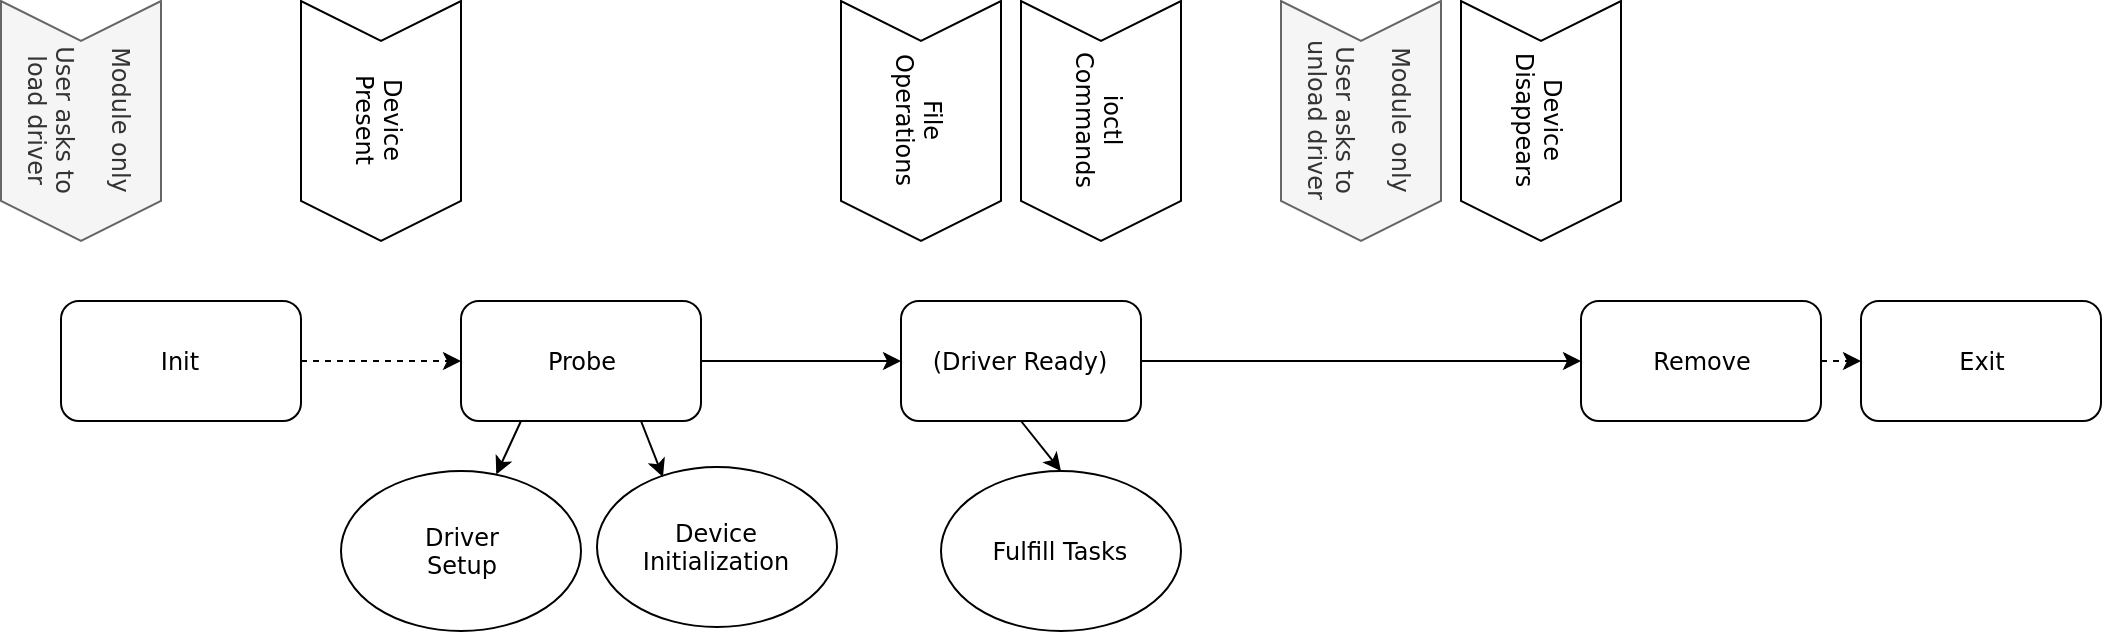
\includegraphics[width=\linewidth]{LinuxDriverLifecycle}
    \caption{Simplified Lifecycle of a Linux Device Driver}
    \label{pic:linux-lifecycle}
\end{figure}

The right information needed to deregister device and the driver's entries for this specific instance should be stored as part of the private per-device datastructure.
Figure~\ref{pic:linux-lifecycle} illustrates this situation.

After probing the device, the driver for this instance is ready for use.
Different interfaces to a driver in Linux were already mentioned in an above section.
Figure~\ref{pic:linux-lifecycle} only pictures the file operations and \texttt{ioctl()} as a special situation within them.
Regardless of the used interface, all corresponding implementations in the driver must be \textit{reentrant}, but not only in terms of different device instances using the same driver code, but also for a single instance receiving multiple requests, e.g.\ from different users.
The implementations task is decoding the user's request, translate it in a command for the device controller and take care of the physical transmission to the device.
Depending on the request, this may includes sending requests for actions, commands and data to the device but also fetching answers, status codes and e.g.\ processed data from it\cite{quade2016Linux}.


\section{Zircon Driver Model}
The driver model in Zircon differs a lot compared to Linux due to the influences of the microkernel approach.
This converns in particular mechanisms and corresponding terms which are used by the system to manage device drivers and enable them in userspace.
Nevertheless, a driver in Zircon has the same purpose as a Linux one: providing a uniform interface to a specific device while its implementation details are hided\cite{zircon-ddk-gettingstarted}. 

\subsubsection*{Device Model}
Zircon's model for devices and drivers is a direct result of choosing a microkernel approach and at the same time a rejection of the situation in Linux.
There, device drivers live in the kernel's address space with privileged access to the whole kernel memory and other resources.
As a result belong each part of the kernel including device drivers to the same process.
A fault isolation within the Linux kernel is not given and a bad driver may break the entire kernel. 
In contrast a pure textbook approach for a microkernel would run each single driver in an own process to reach the maximum possible isolation.
Even if some real-world microkernel implementations do so, it is not an efficient approach as it requires a great amount of context switches and \ac{ipc}\cite{zircon-ddk-gettingstarted}.
Thus, Zircon's idea differentiate from the textbook approach and group a number of related drivers together in so-called \textit{device host} processes\cite{zircon-ddk-gettingstarted}.
A driver itself is in Zircon compiled to a \acf{elf} shared library, a \ac{dso}.

Another related mechanism in the Zircon kernel is the \textit{device manager process (devmgr)}.
It contains the \textit{device coordinator}, a piece of software that keeps track of drivers and devices.
The device coordinator manages the discovery of drivers and devices and is responsible for the cration of device host processes.
A \ac{dso} driver is loaded into a \textit{device host (devhost)} process and lives there maybe together with other related drivers to reduce needed context switches without soften the microkernel concept too much.
In addition, the coordinator maintains the \textit{device filesystem (devfs)} as a mechanism that enables userspace applications to access a driver and thus, the device too.
Similar to the unified device model in Linux, the Zircon device coordinator views devices as a part of a unified tree structure\cite{zircon-devicemodel},~\cite{zircon-ddk-gettingstarted}.
Branches of this tree are represented by device host processes which consist of devices.
At the current state of Zircon, the policy used to decide which drivers are grouped together for performance reasons and which ones should be placed into seperate device host processes is made based on the underlying physical system.
As a result, each device that is able to represent a physical bus master becomes a device host process and all corresponding child devices are placed into this process.
In future, this policy will may evolve to a more sophisticated concept\cite{zircon-devicemodel}.

In Zircon, device drivers may implement \textit{protocols}, that means C \acp{abi}.
A protocol is a strict interface definition and defines a set of functions a driver must implement.
Protocols are specific to classes of devices.
As a result, all devices from a type, e.g.\ \ac{pci} devices must implement the same protocol and thus, the same functions.
Zircon differentiates rather in device protocol types such as \textit{\ac{pci}, \ac{usb}, block core or ethermac} than in block, character or network devices.
A protocol is used by child drivers to interact with its parent drivers in a device specific manner.
So it is an interface protocol between different driver layers, and thus commonly different device host processes, for a particular device type or between drivers in the same device host process\cite{zircon-ddk-gettingstarted},~\cite{zircon-devicemodel}.

Additionally, a device can implement \textit{interfaces}.
They represent \textit{\ac{rpc} protocols} which are used by userspace applications or services.
Interfaces are for example the \ac{posix} styled \texttt{open()}, \texttt{close()}, \texttt{read()}, \texttt{write()} or \texttt{ioctl()} functions but also own interfaces defined using the Zircon specific \acf{fidl}\cite{zircon-devicemodel}.

Within the device filesystem (devfs), Zircon devices respectively drivers are grouped in \textit{classes}.
A class represents in this situation a promise to implement certain protocols and/or interfaces.
Devices exist in devfs in a structured way under a topological path according to the scheme \texttt{/dev/class/device/drivername}, e.g.\ \\
\texttt{/dev/pci/00:02:00/intel-ethernet}.
At the time of writing, the names within the class directories, the device identifiers, are unique numbers in a certain pattern\cite{zircon-devicemodel}.
%TODO -> check classes in runnin zircon

% %General
    % \cite{zircon-ddk-gettingstarted}
    % - zircon: use concept of device host
        % - devhost is a process that contains a protocol stack (one or more protocols that work together)
        % -> devhost loads drivers from elf shared libraries (dsos)
        % -> the protocol stack allows the creation of a complete ``driver'' for a device, consisting of platform dependent and platform independent components -> self contained process container
%
\subsubsection*{Driver Lifecycle}
It is currently not possible in Zircon to built drivers in a different way than the built-in \textit{\ac{elf} shared libraries} mentioned before.
They are not loaded into a device host process until it is determined they are actually needed.
This is done using \textit{binding program} which is a part of the driver.
Within the driver, it is defined using system internal macros.
The compiler moves this program into the \textit{ELF NOTE} section of the binary where it can be inspected by the \textit{device coordinator} without the need to fully load the driver into its own process.
Besides the bind discription itself, the binding program also contains pointers to the most neccessary driver methods\cite{zircon-devicemodel}.

The first but less used method in the Zircon device driver lifecycle is \texttt{init()}.
It is invoked when a driver is loaded into a device host process and used for any global initializations.
While its pedant in Linux is often replaced using macros to reduce boilerplate code, Zircon makes it optional to implement it.
Typically, no implementation for \texttt{init()} is required but if the method is implemented and fails, the whole driver fails\cite{zircon-devicemodel}.
Thus, it is not pictured in the simplified Zircon driver lifecycle in figure~\ref{pic:zircon-lifecycle}.

Similar to Linux' \texttt{probe()} function follows in Zircon the \texttt{bind()} method in a drivers life.
It is invoked by the device coordinator how offers the driver a device to bind.
This device matches the rules the driver has published as a part of its bind program.
Within \texttt{bind()}, the driver has to initialize the device, setup interfaces to itself and publish one or more childs or the device to succeed\cite{zircon-gettingstarted}.
Adding such a child device is done using \texttt{device\_add()}.
It creates a new device and adds it as a child to a provided parent device.
This parent must either be exactly the device which is passed to \texttt{bind()} by the device coordinator or another device which already has been created by the same device driver.
This method includes adding the newly created device to the device filesystem (devfs) which is maintained by the device coordinator.
As soon as a device is added to devfs, the device operations, e.g. \texttt{read()}, \texttt{write()} or calls defined using \ac{fidl}, can be called by the device host.
Figure~\ref{pic:zircon-lifecycle} pictures the simplified situation.
If a device shall be added but not be accessed already, e.g.\ to do a longer initialization as a background thread, the device can also be added in an invisible mode using a specific flag.
After the initialization is done, the device must be made visible to be accessed\cite{zircon-devicemodel}.

The device driver method \texttt{create()} is only invoked for platform or system bus drivers or proxy drivers.
Thus, it concerns only the fewest drivers and is not further considered in this work or the related figure\cite{zircon-devicemodel}.

\begin{figure} [ht]
    \centering
    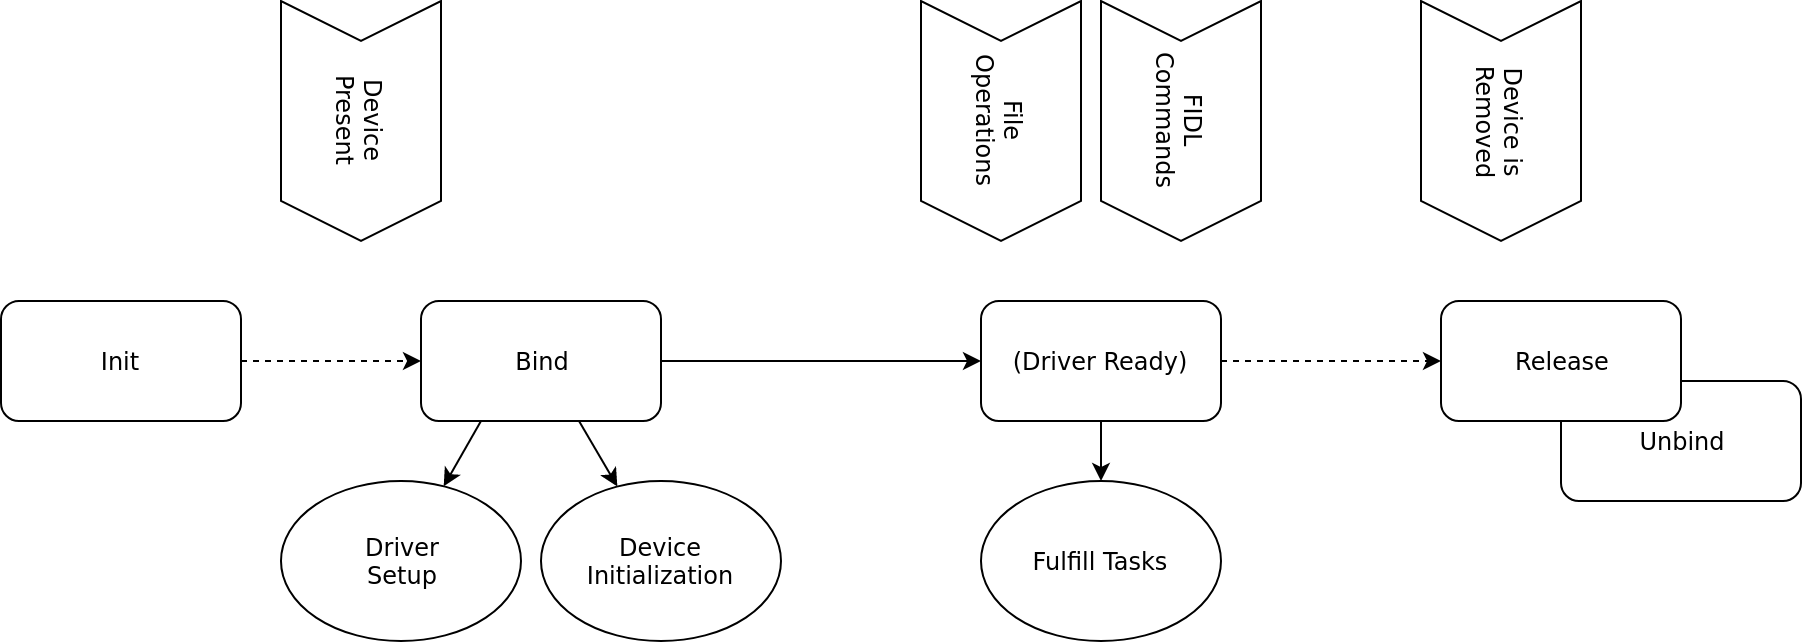
\includegraphics[width=\linewidth]{ZirconDriverLifecycle}
    \caption{Simplified Lifecycle of a Zircon Device Driver}
    \label{pic:zircon-lifecycle}
\end{figure}


The driver's \texttt{release()} method is invoked right before the driver is unloaded and after all devices it may have created in \texttt{bind()} using \texttt{device\_add()} have been destroyed.
The method is never invoked currently because once a driver is loaded, it remains loaded for the lifetime of a device host process.
Nevertheless, it should be implemented.

In theory, \texttt{release()} and the related \texttt{unbind()} method should be called e.g.\ if a parent device detects the corresponding device is removed and thus, calls \texttt{device\_remove()}.
In consequence, the \texttt{unbind()} method is called on all child devices because the parent becomes removed.
Unbind should remove all interfaces that were created in relation to the \texttt{device\_add()} call.
If a device still has work in progress when \texttt{unbind()} is called by the parent, the child device continues this first.
Thus, the parent must ensure the device is not working anymore before it also calls \texttt{release()} as a last step in this exemplarily tear down sequence on all children\cite{zircon-devicemodel}.
%TODO better lifecycle graphic, reference for the last section



\section{Test Setup}

\subsection{Hardware Issues}
% 1.8 vs 5V
%
% The RGB LCD has 2 chips with 2 different functionalities. One of it drives the LEDs and the other one drives the text that’s printed.
%
% The text driver is one and only and has an address of 0x3e.
%
% The LED driver has multiple addresses, of which we only need one. As it’s specified on page 8 (annex 7.1.1) in this datasheet (aka PCA9633) 9, there are 3 fixed addresses for our 8-pin chip package (the PCA9633):
%
% address 0x70 - LED all call address - it’s on at startup and cannot be addressed individually
%
% address 0x03 - Software reset address - it’s on at startup and cannot be addressed individually
%
% address 0x62 - Slave address - it’s the one you are communicating with and is addressable
%
% raspi pi@raspberrypi:~\$ i2cdetect -y 1
    % 0  1  2  3  4  5  6  7  8  9  a  b  c  d  e  f
% 00:          03 -- -- -- -- -- -- -- -- -- -- -- --
% 10: -- -- -- -- -- -- -- -- -- -- -- -- -- -- -- --
% 20: -- -- -- -- -- -- -- -- -- -- -- -- -- -- -- --
% 30: -- -- -- -- -- -- -- -- -- -- -- -- -- -- 3e --
% 40: -- -- -- -- -- -- -- -- -- -- -- -- -- -- -- --
% 50: -- -- -- -- -- -- -- -- -- -- -- -- -- -- -- --
% 60: -- -- 62 -- -- -- -- -- -- -- -- -- -- -- -- --
% 70: 70 -- -- -- -- -- -- --
%
%
% root@linaro-developer:~# i2cdetect -y -r 0
    % 0  1  2  3  4  5  6  7  8  9  a  b  c  d  e  f
% 00:          -- -- -- -- -- -- -- -- -- -- -- -- --
% 10: -- -- -- -- -- -- -- -- -- -- -- -- -- -- -- --
% 20: -- -- -- -- -- -- -- -- -- -- -- -- -- -- -- --
% 30: -- -- -- -- -- -- -- -- -- -- -- -- -- -- -- --
% 40: -- -- -- -- -- -- -- -- -- -- -- -- -- -- -- --
% 50: -- -- -- -- -- -- -- -- -- -- -- -- -- -- -- --
% 60: -- -- 62 -- -- -- -- -- -- -- -- -- -- -- -- --
% 70: 70 -- -- -- -- -- -- --
%
% https://www.kernel.org/doc/Documentation/i2c/instantiating-devices
% https://www.kernel.org/doc/Documentation/i2c/writing-clients
% https://raw.githubusercontent.com/torvalds/linux/v4.20/include/linux/i2c.h
% https://i2c.wiki.kernel.org/index.php/OF_Modalias



\section{General Driver Concept}\label{sec:cs-driver-concept}


\section{Linux}\label{sec:cs-linux}


\subsection{Driver Implementation} %TODO better titel, label
\subsubsection{Interface} %ioctl
    % Development setup for x86-64, ARM64, ...
